\subsubsection{Macro-caso d'uso - Discovery}
\paragraph{Diagramma UML}

\begin{figure}[H]
    \centering
    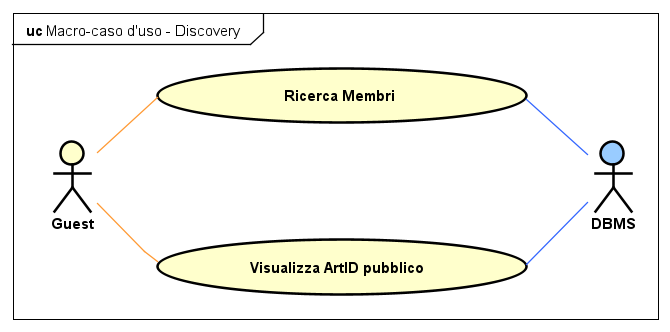
\includegraphics[width=0.95\textwidth, height=0.95\textheight, keepaspectratio]{Immagini/Use-case diagrams/Macro-caso d'uso - Discovery.png}
\end{figure}

\clearpage

\paragraph{Ricerca Membri}
\par{\noindent Questo caso d'uso permette a un Guest di cercare i profili pubblici dei Membri e di consultare gli ArtID pubblici da loro creati.}

\begin{tabularx}{\textwidth}{|C|X|}
\hline
\rigaTabella{Caso d'uso}{Ricerca Membri}
\rigaTabella{ID}{DISC\_MEM}
\rigaTabella{Attori}{Guest, DBMS}
\rigaTabella{Precondizione}{Il sistema ha mostrato la schermata ``WELCOME''}
\rigaTabella{Flusso degli eventi}{\begin{enumerate}
    \item Il Guest clicca sul pulsante ``ESPLORA''
    \item Il sistema mostra la schermata ``ESPLORA''
    \item Il Guest utilizza la barra di ricerca per cercare un Membro in base al nome \label{guest cerca}
    \item Il sistema interroga il DBMS per ottenere i Membri con il nome cercato che abbiano un profilo pubblico, nonch\'e il numero di ArtID con visualizzazione pubblica da questi creati
    \item Il sistema mostra a schermo i risultati
    \item Il Guest clicca su un Membro
    \item Il sistema interroga il DBMS per ottenere tutte i certificati pubblici del Membro
    \item Il sistema interroga il DBMS per ottenere informazioni sugli ArtID con visualizzazione pubblica creati dal Membro
    \item Il sistema mostra la pagina ``ESPLORA PROFILO'' con i dati del Membro selezionato e degli ArtID con visualizzazione pubblica associati
\end{enumerate}
}
\rigaTabella{Sequenze alternative}{
\begin{enumerate}[label=5.]
    \item Il Guest pu\`o ripetere la ricerca se desiderato. In questo caso il caso d'uso riprende dal punto \ref{guest cerca} del flusso principale.
\end{enumerate}
}
\rigaTabella{Postcondizione}{Il sistema ha mostrato a video la schermata ``ESPLORA PROFILO''}
\rigaTabella{Note}{La ricerca pu\`o avvenire anche solo per parte del nome. Il sistema mostrer\`a i risultati pi\`u attinenti.}
\hline
\end{tabularx}

\clearpage

\paragraph{Visualizza ArtID pubblico}
\par{\noindent Questo caso d'uso permette a un Guest di visualizzare i contenuti completi di un determinato ArtID pubblico e le informazioni sul suo autore, a partire dal profilo pubblico del Membro.}

\begin{tabularx}{\textwidth}{|C|X|}
\hline
\rigaTabella{Caso d'uso}{Visualizza ArtID pubblico}
\rigaTabella{ID}{VIS\_ARTID\_PUB}
\rigaTabella{Attori}{Guest, DBMS}
\rigaTabella{Precondizione}{Il sistema ha mostrato la schermata ``ESPLORA PROFILO'' contenente almeno un ArtID pubblico di un Membro con profilo pubblico.}
\rigaTabella{Flusso degli eventi}{\begin{enumerate}
    \item Il Guest clicca su un ArtID
    \item Il sistema interroga il DBMS per ottenere i contenuti dell'ArtID
    \item Il sistema ottiene le informazioni sul Membro autore
    \item Il sistema mostra la pagina ``ARTID PREVIEW - GUEST'' con i contenuti dell'ArtID e informazioni sull'autore
\end{enumerate}
}
\rigaTabella{Postcondizione}{Il sistema ha mostrato a video la schermata ``PREVIEW ARTID - GUEST''}
\hline
\end{tabularx}

\clearpage